\documentclass[12pt]{article}
\usepackage[utf8]{inputenc}	
\usepackage[catalan]{babel}
\usepackage{subcaption}
\usepackage[obeyspaces]{url}
\usepackage[colorinlistoftodos]{todonotes}
\usepackage[]{mcode}
\usepackage{fancyvrb}
\usepackage{eurosym} %Símbol del euro
\usepackage[obeyspaces]{url} %PATH
\usepackage{wrapfig} %Imatges WRAP (mateixa linia)
\usepackage[toc,page]{appendix}
\usepackage{todonotes}
\usepackage{appendix}
\usepackage{scrextend}
\usepackage{enumitem}
\usepackage{dirtytalk}
\usepackage{multicol}
\usepackage{listingsutf8}
\usepackage{dirtytalk}
\usepackage{float}
\usepackage{url}

\setlength{\parindent}{0cm} \setlength{\oddsidemargin}{-0.5cm} \setlength{\evensidemargin}{-0.5cm}
\setlength{\textwidth}{17cm} \setlength{\textheight}{23cm} \setlength{\topmargin}{-1cm} \addtolength{\parskip}{2ex}

\definecolor{backcolour}{rgb}{0.95,0.95,0.92}
\lstdefinelanguage{json}{
	backgroundcolor=\color{backcolour},   
	breaklines=true, 
    string=[s]{"}{"},
    stringstyle=\color{blue},
    comment=[l]{:},
    commentstyle=\color{black}
}

\renewcommand{\baselinestretch}{1.5}

\begin{document}
\begin{titlepage}
		\centering
		\includegraphics[width=0.5\textwidth]{imatges/logo3.png}\par\vspace{1cm}
		{\huge\bfseries Posicionament de restaurants\par}
		\vspace{0.3cm}
		{\scshape\Large Processament de Dades Espaials\par}
		\vspace{0.2cm}
		{\scshape\Large Màster en enginyeria informàtica\par}
		\vspace{1.5cm}
		{\Large\itshape Oscar Galera Alfaro i Meriem Abjil Bajja\par}
		\vfill
		{\large \today\par}
\end{titlepage}
\tableofcontents

\clearpage

\listoffigures

\clearpage

\section{Introducció}

Els dissenyadors de \textit{Disney Land París} han descobert com mantenir el seu univers feliç el més petit possible: mitjançant l'ús de polseres \textit{Magic Bands} per fer un seguiment de les identitats, els moviments i l'estat financer dels usuaris.

El \textit{MyMagic } + \say{sistema de gestió de vacances} pot fer un seguiment dels convidats a mesura que es mouen per \textit{Disney Land París} i analitzar els seus hàbits de compra.

Degut a l'èxit generat per \textit{Disney Land París} (a partir d'ara \textit{DPL}), el propietari d'aquest ha decidit obrir un nou parc temàtic similar (veure \textit{Figura \ref{fig:disney1}}) però aquest cop en el territori Gironí. Ens han encarregat indicar el posicionament dels restaurants amb l'objectiu de maximitzar els beneficis generats per aquests. Per ubicar aquests restaurants, es realitzarà un estudi de la popularitat de les atraccions que hi ha a \textit{DLP} a fi de determinar les zones més visitades, i d'aquesta manera, fer la distribució dels restaurants més cars en aquestes zones per maximitzar els beneficis del parc.

%Posicionament de la imatge
\begin{figure}[H]
    \centering
    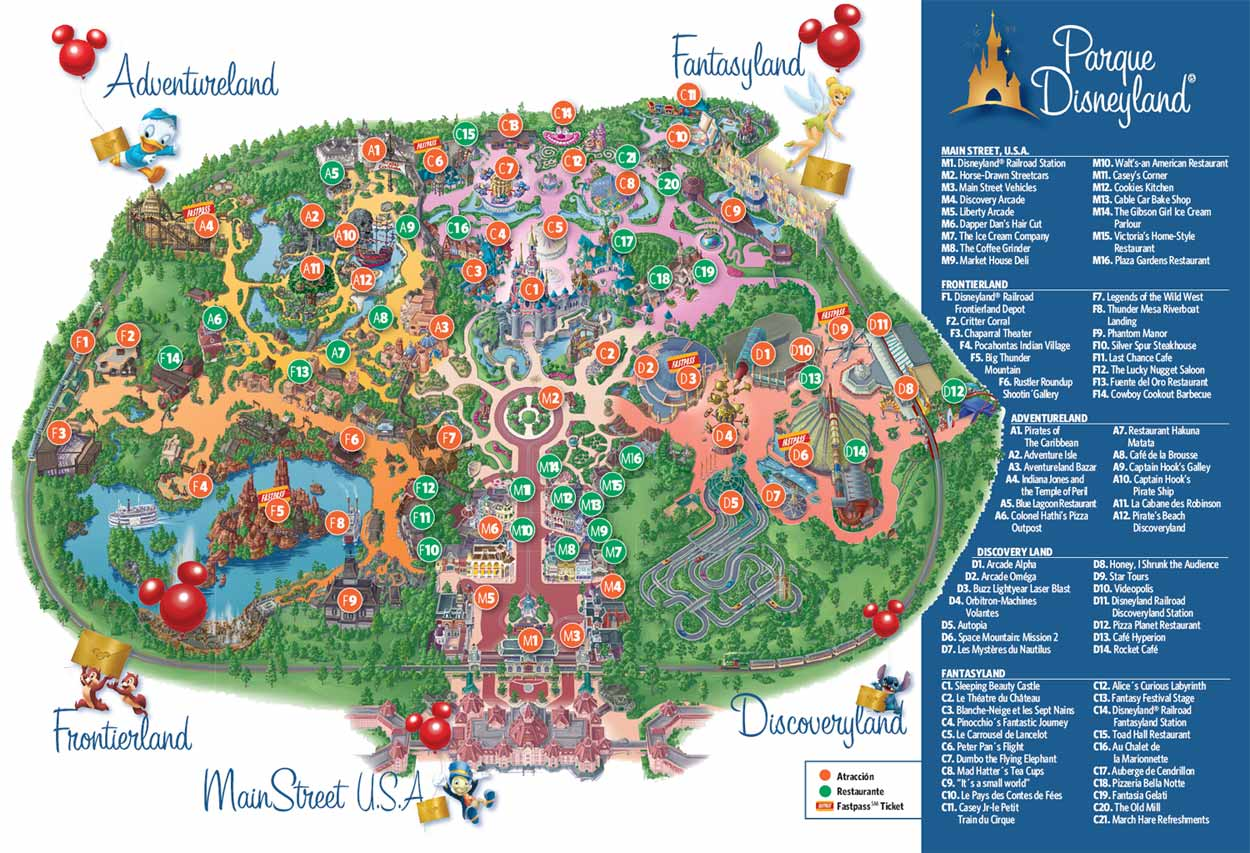
\includegraphics[width=0.75\textwidth]{imatges/mapa_disney_land_paris.jpg}\par\vspace{1cm}
    \caption{Mapa de \textit{Disney Land París}}
    \label{fig:disney1}
\end{figure}

\clearpage
\section{Objectiu}
L'objectiu del projecte és \textbf{fer la distribució dels restaurants més cars a partir d'unes determinades zones \say{remarcades} per maximitzar els beneficis del parc}. Aquestes zones les anomenarem candidates, i seran aquelles on es podran ubicar els restaurants.

Per aconseguir aquest objectiu es considerarà que el mapa d'atraccions del nou territori és el mateix que el de \textit{DLP}; que les \textit{Magic Bands} (veure \textit{Figura \ref{fig:magic_bands}}) recullen i emmagatzemen la informació de la posició dels seus usuaris cada 5 minuts, i que disposem de tantes zones candidates (o més) com restaurants es vulguin ubicar. 

Per determinar el grau d'interès de cada atracció, es compta amb una gran quantitat de dades generades per les \textit{Magic Bands} (veure \textit{Figura \ref{fig:magic_bands}}) que es reparteixen a l'entrada del parc temàtic, i que tenen per objectiu la recollida de dades per l'estudi del comportament del públic. 

\begin{figure}[H]
    \centering
    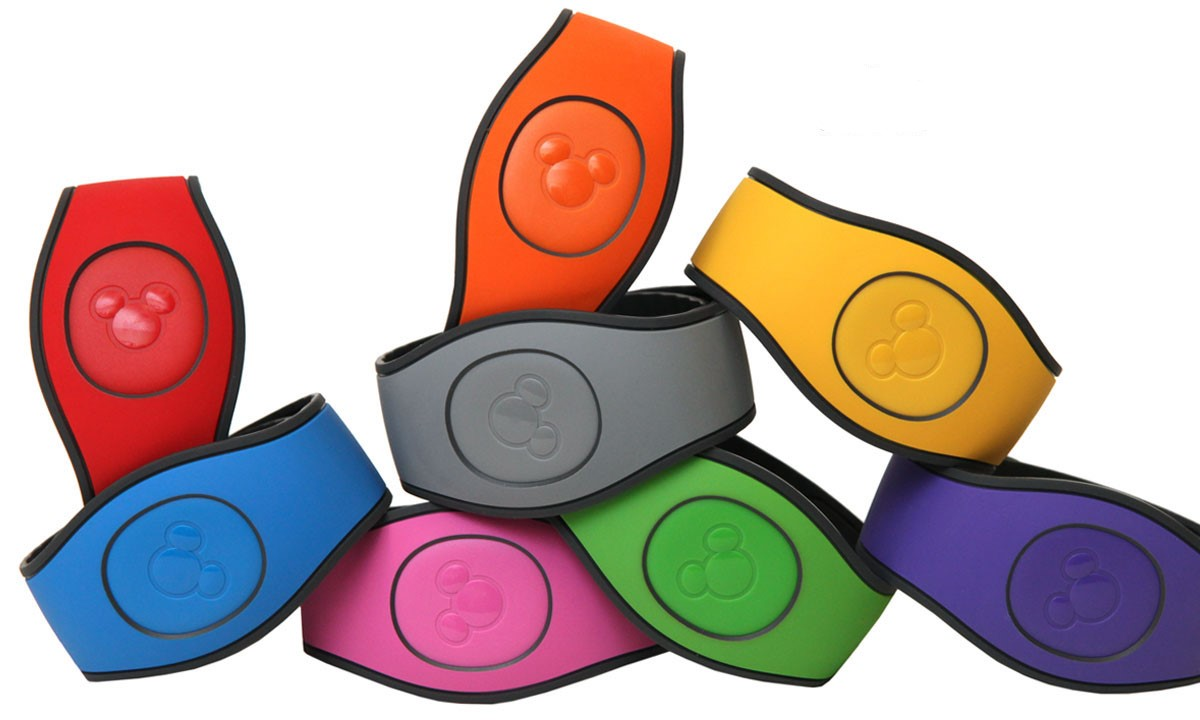
\includegraphics[width=0.75\textwidth]{imatges/magic_bands.jpg}\par\vspace{1cm}
    \caption{\textit{Magic Bands}}
    \label{fig:magic_bands}
\end{figure}

\clearpage
\section{Definició del problema}
Així doncs, per aconseguir l'objectiu que s'ha plantejat es seguiran 6 passos, que són:
\begin{enumerate}
	\item Preprocessament de dades (veure \textbf{secció \ref{pd}}).
	\item Filtrat de dades.
	\item Assignar un pes a cada atracció.
	\item Dividir el mapa en àrees.
	\item Calcular la importància de cada atracció.
	\item Definir les zones candidates.
	\item Ubicar els restaurants.
\end{enumerate}

S'assumeixen les següents entrades:
\begin{itemize}
	\item Un fitxer amb els punts\footnote{Els punts es defineixen per la latitud i la longitud.} que defineixen els límits del mapa, juntament amb els punts on hi ha situades les entrades de les atraccions i la quantitat de gent que hi ha pujat.
	\item Un fitxer amb les zona prohibida\footnote{Per zona prohibida s'enten l'àrea que cobreixen les atraccions, així com els obstacles típics que es poden trobar en un parc d'atraccions.} definides pels seus punts i arestes (s'assumeix que les àreas estan definides per poligons).
	\item Un fitxer amb els punts que representen les persones i la hora en què s'han recollit.
\end{itemize}

\subsection{Filtrat de dades}
En aquest apartat es volen filtrar els punts de les persones situades en àrees prohibides. Per això, es crearà una estructura \textit{PM QuadTree} a partir dels poligons que regeixen els obstacles i que s'usarà per eliminar tots aquells punts que es trobin a dins.

Per construir el PM Quadtree s'utilitzarà el següent algoritme:

EXPLICACIÓ DE L'ALGORTME PM QUADTREE (MERIEM)

Un exemple de l'aplicació d'aquesta estructura es pot veure en la següent \textit{Figura \ref{fig:poligon_pm_quadtree}}:

\begin{figure}[H]
	\centering
	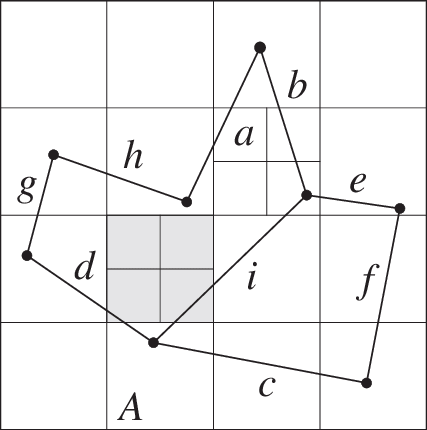
\includegraphics[width=0.5\textwidth]{imatges/pm_quadtree.png}\par\vspace{1cm}
	\caption{Poligon emmagatzemat en un PM Quadtree}
	\label{fig:poligon_pm_quadtree}
\end{figure}

FALTA EXPLICACIÓ DE L'EXEMPLE AMB L'ALGORISME (MERIEM)

Un cop es té creada l'estructura, s'avaluarà cada un dels punts per veure en quina regió està. Si aquesta regió conté part d'un obstacle s'haurà de comprobar si el punt està o no dins d'aquest. Si el punt no es troba dins d'un obstacle, es considerarà una dada vàlida i es posicionarà a sobre d'una grid, de manera que, a la grid tindrem posicionades totes les dades vàlides.

IMATGE GRID AMB ELS PUNTS (MERIEM)

\subsection{Assignar un pes a cada atracció}
El pes d'una atracció es definirà a partir de la quantitat de gent que ha pujat a aquesta. Per cada pivot, s'assigna un pes $p_{i}$ tal que:
 
$$p_{i} = \frac{q_{i}}{t}$$

on:
\begin{itemize}
	\item $q_{i}$ és la quantitat de gent que ha pujat a l'atracció $i$.
	\item $t$ és el total de gent.
\end{itemize}

En la següent \textit{Figura \ref{fig:mapa_areas}} es pot veure el mapa amb el pes per a cada una de les atraccions.

\begin{figure}[H]
	\centering
	\includegraphics[width=0.6\textwidth]{imatges/pesos.png}\par\vspace{1cm}
	\caption{Pesos de cada atracció}
	\label{fig:mapa_areas}
\end{figure}

MODIFICAR LA IMATGE (FER PONDARACIONS) (OSCAR)

\subsection{Dividir el mapa en àrees \label{arees}}
A partir del pes de cada atracció (ubicat en l'entrada d'aquesta), es poden seguir diferents estratègies per calcular la regio d'influència per cada una de les atraccions a partir del nombre de gent del voltant.

\subsubsection{Estratègies}
Algunes d'aquestes estratègies són:
\begin{itemize}
	\item Utilitzar un diagrama de \textit{Voronoi} per definir la regió d'interès de cada atracció (cada persona dins d'aquesta àrea computa 1).
	\item Utilitzar l'estratègia del punt anterior, i per cada atracció, per cada una de les àreeas no definides pel pivot, computar les persones que hi ha com $\frac{1}{1+d}$ on $d$ correspon a la distància en metres des de la persona a l'entrada de l'atracció.
	\item Utilitzar la estratègia del punt anterior, però aquesta vegada comptant la distància ($d$) des de la persona al segment que defineix l'àrea regida pel pivot.
	\item Utilitzar diagrames de \textit{Voronoi} de nivell amb capa ($k$ on $2 \le k \le n$ i $n$ és el nombre d'atraccions), el diagrama de primer nivell defineix la regió de màxim interés de l'atracció (computant 1 per cada persona) i les capes $k-1$ \textbf{capes superposades}, determinen zones d'interès però no tan importants (computen $\frac{1}{k}$ per cada persona).
\end{itemize}

Segons l'estratègia que es volgués seguir, s'obtindria una distribució en àrees o un altre. En aquest cas, s'ha obtat per utilitzar l'última proposta amb una $k = 2$, ja que es creu que és una bona aproximació pel problema que es vol resoldre. 

MOURE A L'ANNEX (OSCAR)

DESDE AQUI....
Quan es parla dels diagrames de \textit{Voronoi} es fa referència a una estructura geomètrica que representa informació de proximitat sobre un conjunt de punts. Els diagrames de \textit{Voronoi} són una de les estructures fonamentals dins de la Geometria Computacional, d’alguna manera emmagatzemen tota la informació referent a la proximitat entre punts.

Però què és un diagrama de \textit{Voronoi}? Per tal d’entendre més ràpidament el concepte introduirem els diagrames de \textit{Voronoi} sobre el pla.

En la següent \textit{Figura \ref{fig:regio_voronoi}} podem veure que el punt $x$ està dins de la regió de punts més propers a $p$. Aquesta regió és la regió de \textit{Voronoi} del punt $p$, i $p$ és el punt generador de la regió.

\begin{figure}[H]
	\centering
	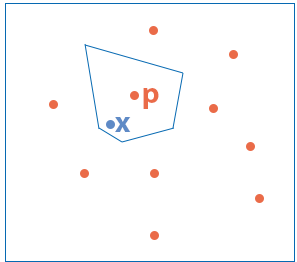
\includegraphics[width=0.3\textwidth]{imatges/regio_voronoi.png}\par\vspace{1cm}
	\caption{Regió \textit{Voronoi}}.
	\label{fig:regio_voronoi}
\end{figure}

La unió de totes les regions de \textit{Voronoi} formen el diagrama de \textit{Voronoi}, tal i com podem veure a la \textit{Figura \ref{fig:diagrama_voronoi}}

\begin{figure}[H]
	\centering
	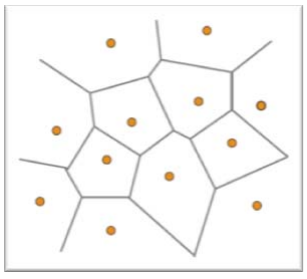
\includegraphics[width=0.3\textwidth]{imatges/diagrama_voronoi.png}\par\vspace{1cm}
	\caption{Diagrama de \textit{Voronoi}}.
	\label{fig:diagrama_voronoi}
\end{figure}

FINS AQUI

Un cop entès el concepte (veure Annex ) del que és un diagrama de \textit{Voronoi} sobre el pla, podem aplicar els mateixos conceptes sobre el nostre projecte. 

A partir de la funció distància de cada punt es poden obtenir diferents diagrames de \textit{Voronoi}: el més proper i el segon més proper. 

Per trobar els diferents diagrames de \textit{Voronoi}, cal definir de quina manera es calcularan les distàncies entre dos punts. Per calcular la distància entre un punt i un pivot s'utilitarà l'\textbf{alogirtme A*} per cada punt de la grid, de manera que el primer pivot que troba es considera el punt generador més proper i el segon punt que troba es considera el segon punt generador més proper.

ANNEX 2. ALGORITME A* (MERIEM) (PSEUDOCODI) 

Desde cada punt situat a la grid es trobarà el primer i segon pivot més proper tenint en compte que a la grid hi han camins habilitats i no habilitats (els camins no habilitats corresponen als camins on es troba un obstacle). Per això, abans d'aplicar A*, aplicarem l'\textbf{algoritme Dijkstra} sobre la grid començant des d'un pivot per eliminar tots els camins que no estan habilitats, és a dir, que hi hagin obstacles.

\subsubsection{Diagrama de \textit{Voronoi} de primer nivell} 

En la següent \textit{Figura \ref{fig:diagrama_voronoi_ordre_1}} es pot veure una possible representació del diagrama de \textit{Voronoi} d'ordre 1.

\textbf{Falta posar els poligons que regeixen les zones prohibides, rius, llacs, les propies atraccions...} (MERIEM)
1
\begin{figure}[H]
	\centering
	\includegraphics[width=1\textwidth]{imatges/diagrama_voronoi_ordre_1.png}\par\vspace{1cm}
	\caption{Diagrama de \textit{Voronoi} d'ordre 1}.
	\label{fig:diagrama_voronoi_ordre_1}
\end{figure}

\subsubsection{Capa de \textit{Voronoi} de primer nivell capa 2}
Per afinar més els càlculs, es vol calcular la capa 2 del diagrama de \textit{Voronoi} de primer nivell, i a partir d'aquesta obtenir una aproximació de la influència de les persones que estan pròximes a l'àrea definida en el primer nivell.

Per obtenir la capa 2, cal realitzar l'algoritme del \textbf{diagrama de \textit{Voronoi} de primer nivell capa 2} utilitzant, com a pivot del diagrama de \textit{Voronoi}, el segon pivot més proper.

%En la següent figura (\ref{fig:diagrama_voronoi_ordre_2}) es pot veure el diagrama de \textit{Voronoi} de primer nivell capa 2, el qual superposant-lo amb el diagrama de \textit{Voronoi} de primer nivell, s'obtindria la capa de superposició que es vol.

%Superposant el diagrama de \textit{Voronoi} de segon nivell amb el diagrama de \textit{Voronoi} de primer nivell, s'obtindria la capa de superposició que es vol.

%\textbf{Falta posar els poligons que regeixen les zones prohibides, rius, llacs, les propies atraccions...}

%\begin{figure}[H]
	%\centering
	%\includegraphics[width=1\textwidth]{imatges/diagrama_voronoi_ordre_2.png}\par\vspace{1cm}
	%\caption{Diagrama de \textit{Voronoi} d'ordre 2}.
	%\label{fig:diagrama_voronoi_ordre_2}
%\end{figure}

\subsection{Definir les zones candidates}
Un cop es disposa de la regió d'influència de cada atracció (veure Secció \ref{arees}). Es vol fer el posicionament dels restaurants, però abans cal que la direcció del parc proporcioni un mapa tot indicant quines són les possibles ubicacions per aquests restaurants. En la següent \textit{Figura \ref{fig:zones_candidates}} es mostra un possible mapa.

\begin{figure}[H]
	\centering
	\includegraphics[width=0.9\textwidth]{imatges/possibles_ubicacions.png}\par\vspace{1cm}
	\caption{Mapa amb les possibles ubicacions}.
	\label{fig:zones_candidates}
\end{figure}

\subsection{Ubicar els restaurants}
En aquest punt, la direcció ha de proporcionar una llista amb els restaurants que es volen ubicar amb un valor associat, aquest valor ha de reflexar quant car és cada restaurant.

Una vegada es tenen els restaurants a ubicar i les zones candidates, cal calcular el benefici de cada configuració a partir del benefici de cada restaurant i la influència que rep en base a les atraccions que té al voltant.  

PER CALCULAR EL BENEFICI DE CADA CANDIDAT:
- DEFINIM L'ÀREA CIRCULAR QUE COBREIX UN RESTAURANT
- CALCULEM L'ÀREA PONDERADA A PARTIR DEL PES DELS PIVOTS DELS DIAGRAMES DE VORONOI SUPERPOSATS DE CAPA 1 I CAPA 2

EXPLICACIÓ D'UN EXEMPLE DE CALCUL DEL BENEFICI (MERIEM)

Una vegada generada totes les combinacions, s'elegirà la que maximitzi el benefici global del parc. En la següent \textit{Figura \ref{fig:mapa_restaurants}} es mostra un exemple d'una possible solució.

\begin{figure}[H]
	\centering
	\includegraphics[width=0.9\textwidth]{imatges/solucio.png}\par\vspace{1cm}
	\caption{Mapa d'atraccions amb les ubicacions dels restaurants}.
	\label{fig:mapa_restaurants}
\end{figure}


\section{Pre-processament de dades\label{pd}}
Pel caràcter del problema i per evitar errors, es realitzarà un preprocessament amb els punts recollits, de tal manera que, només es consideraran els punts que:
\begin{itemize}
	\item S’han recollit dins d’un conjunt de franges horàries que es consideren d'interés pels visitants alhora de buscar un restaurant per anar a menjar. 
	Així doncs, el llistat de franges horàries a considerar és:
	\begin{itemize}
		\item Esmorzar: 9h-10h
		\item Dinar: 12h-14h
		\item Berenar: 17h-18h
		\item Sopar: 20h-22h
	\end{itemize}

	\item No s’hagin recollit a les zones on es troben obstacles. 
	Considerem obstacles a les atraccions, boscos, llacs….
\end{itemize}

Per realitzar-ho, seguirem els següents passos:
\begin{itemize}
	\item Convertir els punts donats (latitud, longitud) que delimiten el mapa en (x,y) a través de l'algoritme XXXXX
	\item Convertir els punts dels pivots (latitud, longitud) i comprovar que estiguin dintre del mapa
	\item Convertir els punts i les arestes de les zones prohibides en (x,y)
	\item Convertir els punts obitnguts de les persones en (x,y):
	\begin{itemize}
		\item Filtrar els punts per l'horari. Només es quedaran els punts de les hores que ens interessen
		\item Convertir els punts filtrats en (x,y)
	\end{itemize}
	
\end{itemize}

\clearpage
\section{Treball futur}
- Programació en paral·lel:
	El calcul de distancies
	Calcul dels diagrames de Voronoi (explicació)

- PER FER ELS CÀLCULS TENIR EN COMPTE DIFERENTS CRITERIS, COM PER EXMEPLE, L'EDAT DELS USUARIS, EL TIPUS D'ATRACCIÓ

- CLUSTERING DE RUTES

\clearpage
\section{Resum del projecte}

L'objectiu principal d'aquest projecte és \textbf{fer la distribució dels restaurants amb l'objectiu de ubicar aquells que són més cars en les zones més freqüentades, per això, es parteix de la informació d'un parc d'atracció similar en el qual s'han recollit les dades dels visitants del parc a través de les \textit{Magic Bands}. L'objectiu d'aquest projecte ha estat complert satisfactòriament. 

ACABAR CONCLUSIONS

\clearpage
\begin{thebibliography}{9}
\bibitem{cert1} \textsc{Gizmodo.com.}, \textit{How I Let Disney Track My Every Move}, 2017. \textcolor{blue}{\url{https://gizmodo.com/how-i-let-disney-track-my-every-move-1792875386}}	
\bibitem{cert2} \textsc{Okabe, A.}; \textsc{Boots, B.}; \textsc{Sugihara, K.}, \textit{Spatial tessellations. Concepts and Aplicattións of \textit{Voronoi} Diagrams 2ºe.d}. \textcolor{blue}{\url{http://www.gbv.de/dms/ilmenau/toc/119618044.PDF}}
\bibitem{cert3} \textsc{Abellanas, B.}; \textsc{Abellanas, M.}; \textsc{Vilas, C.}, \textit{Modelización de bosques mediante diagramas de \textit{Voronoi}}, 2018. \textcolor{blue}{\url{https://www.infor.uva.es/egc07/articulos/28.pdf}}
\bibitem{cert4} \textsc{Moya Carrasco, Á.}, \textit{Generación de trayectorias en tiempo real a partir de diagramas de \textit{Voronoi}}, 2016. \textcolor{blue}{\url{https://idus.us.es/xmlui/bitstream/handle/11441/44404/TFG_Angel_Moya_Carrasco.pdf?sequence=1&isAllowed=y}}
\bibitem{cert5} \textsc{Trinchet Almaguer, D}; \textsc{Pérez Rosés, H.}, \textit{Algoritmo para solucionar el problema inverso generalizado de \textit{Voronoi}}, 2007. \textcolor{blue}{\url{http://www.redalyc.org/pdf/3783/378343634005.pdf}}
\bibitem{cert6} \textsc{García, O.}, \textit{The state-space approach in growth modelling}, 1994. \textcolor{blue}{\url{https://www.researchgate.net/publication/237870252_The_state-space_approach_in_growth_modelling}}
\bibitem{cert7} \textsc{ABC.}, \textit{El diagrama de \textit{Voronoi}, la forma matemática de dividir el mundo}, 2017. \textcolor{blue}{\url{https://www.abc.es/ciencia/abci-diagrama-voronoi-forma-matematica-dividir-mundo-201704241101_noticia.html}}
\end{thebibliography}
\end{document}
